\documentclass[11pt,a4paper]{article}
\usepackage[utf8]{inputenc}
\usepackage[spanish]{babel}
\usepackage{amsmath}
\usepackage{amsfonts}
\usepackage{amssymb}
\usepackage{graphicx} 
\usepackage{lmodern}
\usepackage[left=2cm,right=2cm,top=2cm,bottom=2cm]{geometry}
\author{ Israel Monjaraz Ramírez }
\title{NOTAS 3}
\usepackage{fancyhdr}
\usepackage{float}
\usepackage{listings} 
\usepackage[usenames,dvipsnames,svgnames,table]{xcolor}


\begin{document}
	

	\pagestyle{empty}	 %quitar enumeracion de pag
%	\thispagestyle{empty}
	
	
	
	\begin{tabular}{c}
		{\LARGE \textbf{INSTITUTO POLITÉCNICO NACIONAL}}  \\ 
		{\Large \textsc{\textbf{Escuela Superior de Ingeniería Mecánica y Eléctrica}  } } \\ 
		\textbf{UNIDAD AZCAPOTZALCO }\\ 
		\textbf{INGENIERÍA MECÁNICA} \\
	\end{tabular} 
	\begin{tabular}{c}
		
\includegraphics[scale=0.20125687]{figures/esimeBN}
	\end{tabular}
	
	\lfoot[]{ }
	\cfoot[]{}
	\rfoot[]{ }
	\renewcommand{\headrulewidth}{0pt}
	
	
	
	
	\vspace*{1cm}
	\begin{center}
		\begin{Large}
			\textbf{DESARROLLO PROSPECTIVO DE PROYECTO II}\\[0.2cm ]
			\textit{Cálculo y diseño de una cámara de refrigeración para la conservación de insulina en Santa Bárbara Azcapotzalco Ciudad de México}\\[0.4cm]
			
			%\textbf{\underline{Entrega primer parcial: Capítulo IV}}		
		\end{Large} 
	\end{center}
	\vspace*{1cm}
	\begin{center}
		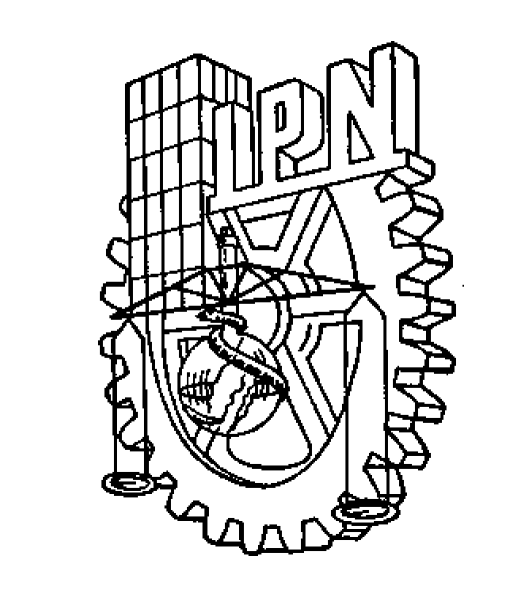
\includegraphics[scale=0.62256022]{figures/ipnlines}\hspace{4cm} 
	\end{center}

	
	
	
	\begin{center}
		\begin{Large}
			\textbf{Entrega:}\\[0.2cm] 
		\end{Large}
		
			{\Large\textit{Israel Monjaraz Ramírez (9MM1)}}\\[0.2cm] 
			2020360966
		
		\begin{Large}
			\textbf{Directores del proyecto:}\\[0.2cm] 
		\end{Large}
		
		
		\begin{tabular}{l}
			Dr.	Alejandro Zacarías Santiago\\
			M en C. Cuauhtémoc Jiménez Castillo\\
		\end{tabular}

		
	\end{center}
	\vspace{0.2cm}
	\begin{center}
		\begin{Large}
			\textbf{Profesores responsables de la asignatura:}\\[0.2cm] 
		\end{Large}
		
		
		\begin{tabular}{l}
			Dr. Soto Muciño Luis Enrique\\
		Ing. Nolasco Quintero Jorge Osvaldo\\
		
		\end{tabular}
		
	\end{center}
	\vspace{0.8cm}
	\begin{flushright}
		\begin{tabular}{|c|}
			\hline
		12.12.2024\\
			\hline
		\end{tabular}
	\end{flushright}

			\section*{Agradecimientos}
	{\itshape
		
		
		A mi madre, cuyo apoyo incondicional, amor y confianza han sido mi motor principal para no rendirme. Su ejemplo de fortaleza y sus palabras de aliento me han guiado en cada paso que he dado. Gracias por creer en mí, incluso en los momentos en los que dudaba de mí mismo. A mi padre, quien en vida fue mi mayor ejemplo de fortaleza, dedicación y amor. Su recuerdo y enseñanzas han sido mi guía en cada paso que doy. Este logro es también suyo.\\
		
		Un agradacimiento a mis hermanos que con su admiración me han impulsado en seguir adelante y mejor como persona y profesionalmente.\\
		
		Y a mí mismo, por haber perseverado frente a las innumerables dificultades y obstáculos que se presentaron en el camino. Hoy, con gran satisfacción, presento este trabajo como uno de los logros más importantes de mi carrera, un reflejo de esfuerzo, dedicación y superación personal. \\
	}
	\begin{flushright}
		(\textit{Israel Monjaraz})
	\end{flushright}
	
	\newpage
	
	
\end{document}

